%
% problemstellung.tex -- Beispiel-File für die Beschreibung des Problems
%
% (c) 2020 Prof Dr Andreas Müller, Hochschule Rapperswil
%
\section{Problemstellung
\label{fem:section:problemstellung}}
\rhead{Problemstellung}
Die Partielle Differentialgleichung (DGL) in der Ebene hat die Form 
\begin{equation}
	\Delta x = \lambda x
	\label{fem:equationPDE}
\end{equation} 

\subsection{Was sind Ansatzfunktionen?}
Um eine gesuchte Funktion als Lösung für die Partielle DGL Problem in der Ebene zu finden, wird diese mit einfacheren Funktionen approximiert. Diese einfacheren Approximations- Funktionen werden in diesem Kapitel als Ansatzfunktion $u(x)$ bezeichnet. Die einzelne ANsatzfunktion ist jedoch keine globale Lösung.

Als einfachere Funktionen bieten sich Polynome mit niedrigem Grad an. Diese sind einfach integrier- und differenzierbar. Der Polynomgrad 1 ist einfach anzuwenden bzw. zu berechnen. Polynomgrade 3 und 4 beispielsweis bieten dafür eine bessere Approximation an. Wie im Kapitel 7 ist auch hier das Ziel Gleichungen mit wenigen Koeffizienten zu erstellen. Ist es nun möglich ebenfalls in der Ebene Ansatzfunktionen zu finden mit wenigen Koeffizienten, obwohl über ein Gebiet integriet wird? Ja. Allerdings gibt es besondere Herausforderungen zu beachten, die in den nächsten Zeilen genauer beschrieben werden.
%Die Ansatzfunktion ist frei wählbar und gibt auch den Freiheitsgrad vor. Je höher die Ordnung der Ansatzfunktion desto besser soll die Approximation werden. So die Hoffnung. Allerdings hat dies auch Konsequenzen, die im Verlauf dieses Kapitels beschrieben werden. 


\subsection{Herausforderung FEM in der Ebene}
Wie auch in der Dimension 1 wird das gesamte Gebiet $\Omega$ bzw. Ebene in Teilgebiete $\Omega_i$ unterteilt. Die Teilgebiete sind einfache geometrische Formen wie z.B. in Abbildung \ref{fig:Figuren}. Unterschiedliche geometrische Formen approximieren unterschiedlich gut die gewünschte Fläche. Als Lösung dienen äquivalente Minimalprobleme sprich anstatt Ableitungen werden Integrale verwendet gemäss Kapitel 7.
\begin{figure}[h!]
	\centering
	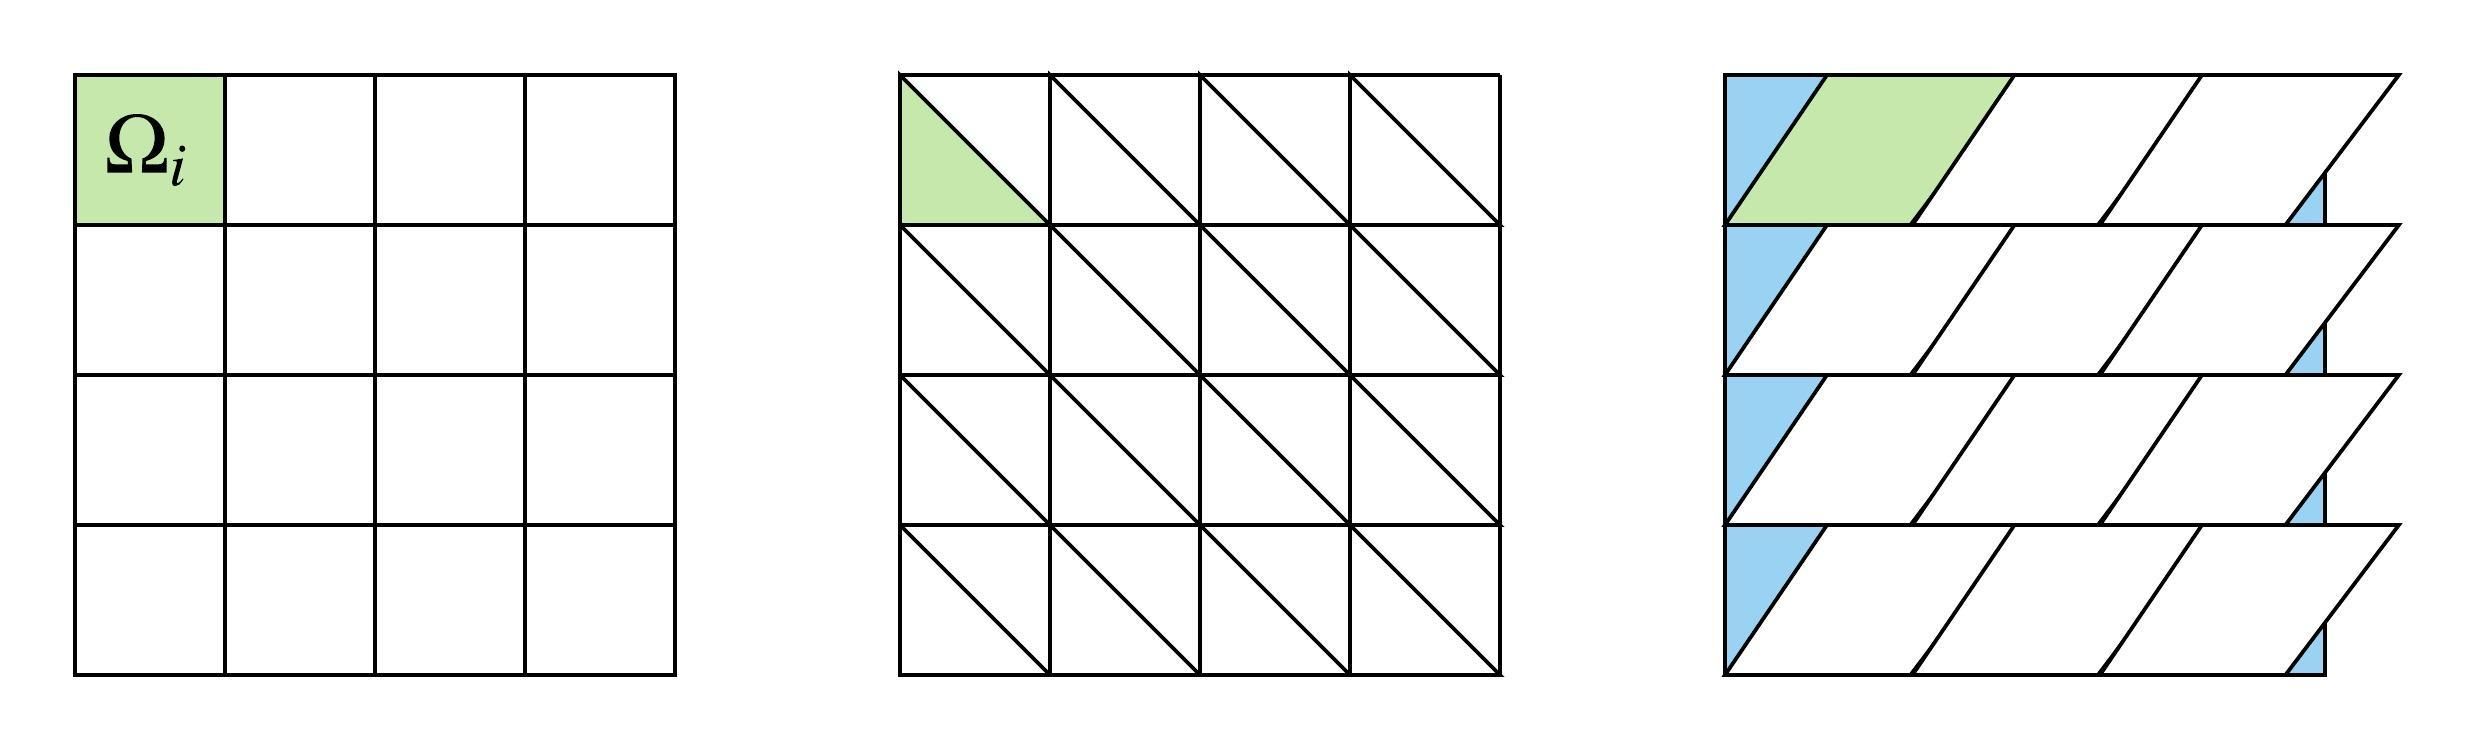
\includegraphics[scale=0.6]{papers/fem/Images/Figuren.jpeg}
	\caption{Approximationsmöglichkeiten eines Qudratischen Gebietes}
	\label{fig:Figuren}
\end{figure}
Damit dies funktioniert müss den die Teilgebiete einfach sein. Auf diese Teilgebiete werden dann die einfachen Ansatzfunktionen angewendet und dann aufsummiert nach \eqref{fem:equationSummGebiete}.

\begin{equation}
\int_{\Omega} (u)^2 \, dx \, dy = \sum \limits_{i=1}^n \int_{\Omega_i} (u)^2 \, dx \, dy 
\label{fem:equationSummGebiete}
\end{equation}
Sollte die Frage auftauchen warum ein Integral mit quadratischen Ausdrücken verwendet wird, so wird auf das Kapitel 7.4.1 verwiesen. Eine Approximation eines gebietes kann Beispielsweise mit Dreiecken, Rechtecken oder Parallelogrammen vorgenommen werden. Aus dieser Approximation resultieren zwei wesentliche Herausforderungen:
\begin{enumerate}
	\item stetig differenzierbar in den Stützstellen (Steigung) wie z.B: im Dreieck in den Ecken.
	\item stetig differenzierbar an den Übergängen entlang den Rändern eines Elements zum anliegenden Rand eines benachbarten Elements. (Krümmung)
\end{enumerate}
Um diese beiden Herausforderungen etwas besser verständlich zu machen wurde  eine Funktion- Approximation dargestellt  $u(x,y) = 1-x^2-y^2$, welche eine Lösung der PDE $\Delta u = -4$ ist mit Randbedingungen $u=0$ auf dem Einheitskreis (violett).
\begin{figure}[h]
	\centering
	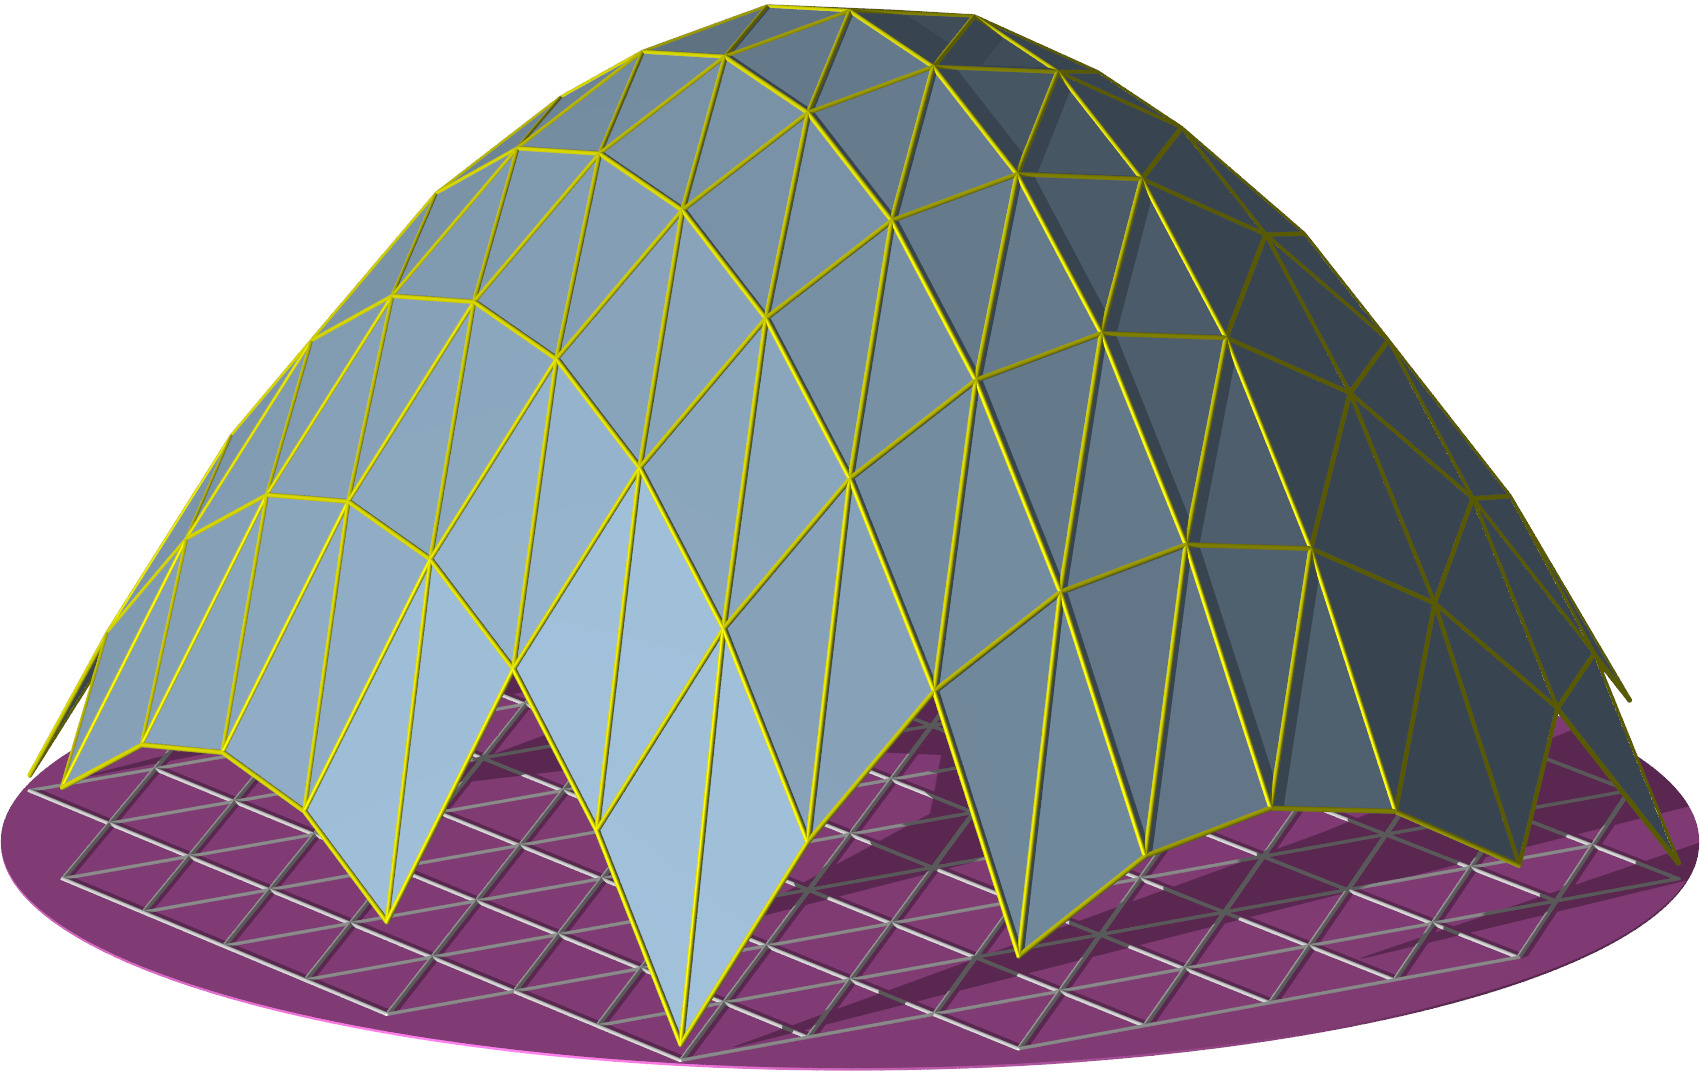
\includegraphics[scale=0.8]{papers/fem/Images/ansatz.jpg}
	\caption{Approximation mit Dreiecken auf einem quadratischen Gitter }
	\label{fig:Ansatz}
\end{figure}
Wie in der Abbildung \ref{fig:Ansatz} zu erkennen ist, passt die Approximation mit Dreiecken auf einem quadratischen Gitter nicht gut, da sich die Randbedingungen nicht ausnutzen lassen. Es benötigt also eine Unterteilung der Kreisscheibe die bis an den Rand kommt. Eine bessere Approximation ist in \ref{fig:besser Approx} zu sehen, die eine bessere Triangulation zeigt.
\begin{figure}[h!]
	\centering
	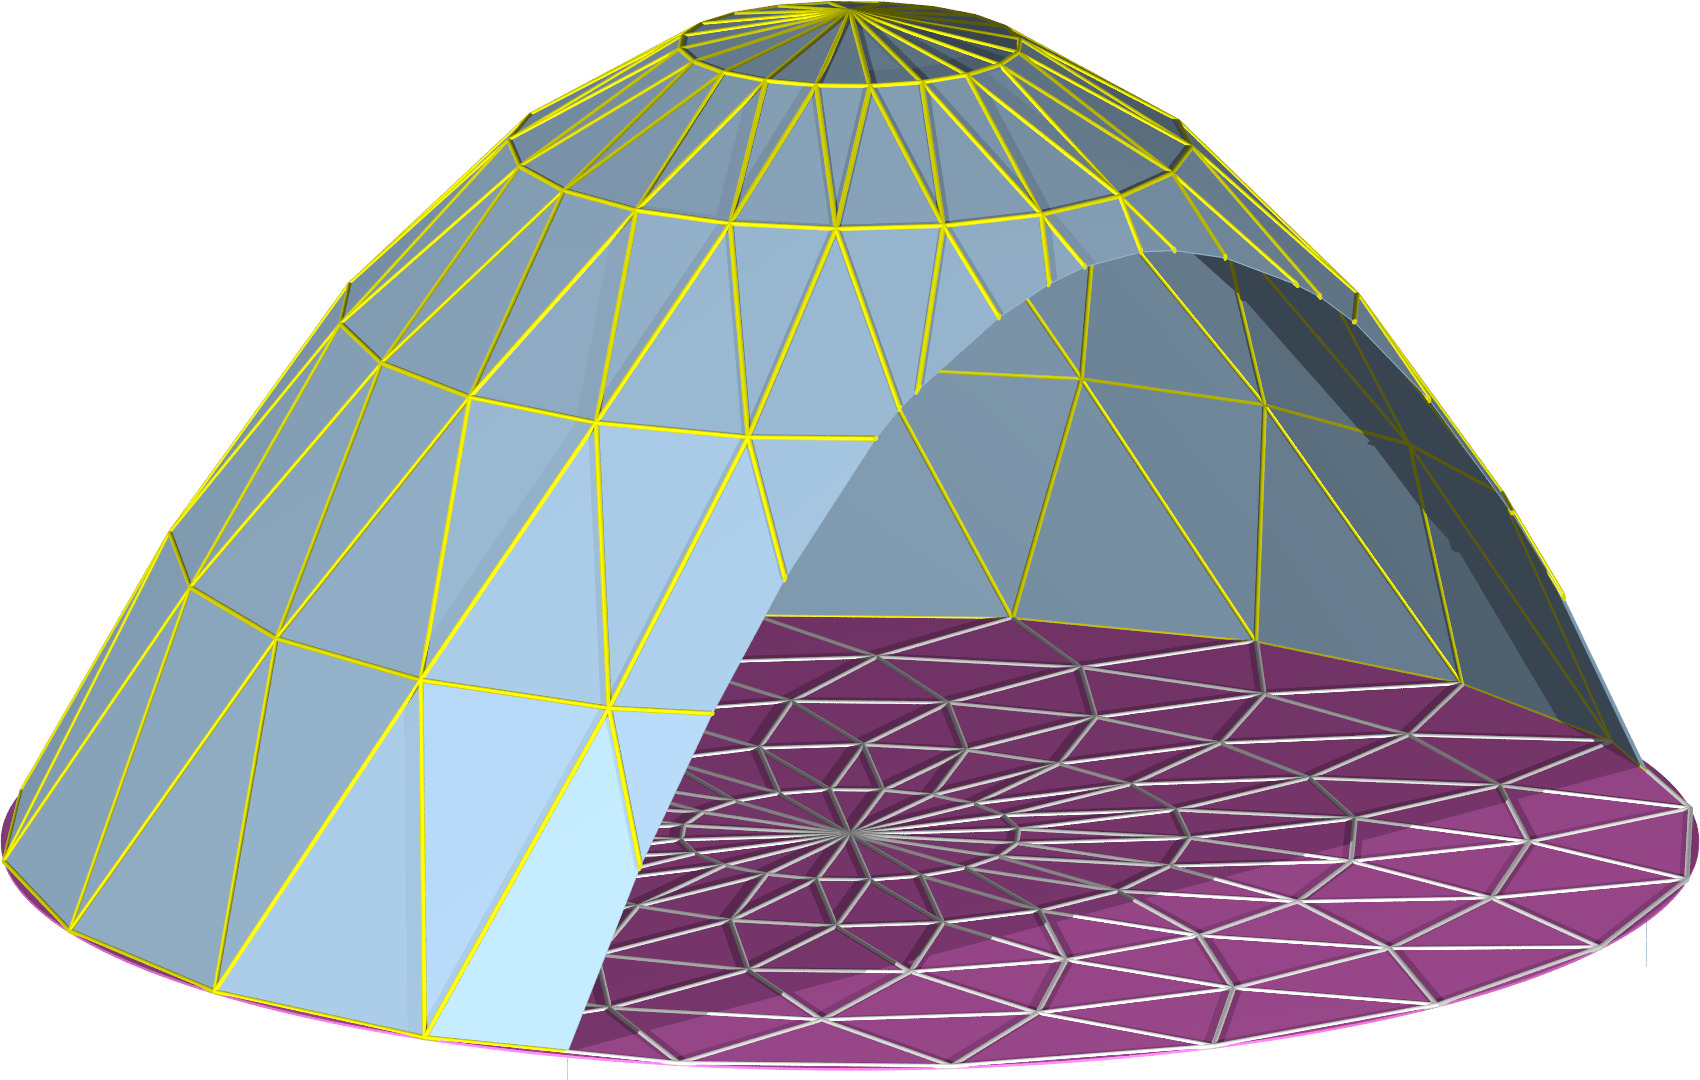
\includegraphics[scale=0.8]{papers/fem/Images/polar.jpg}
	\caption{bessere Triangulation}
	\label{fig:besser Approx}
\end{figure}
\begin{figure}[h]
	\centering
	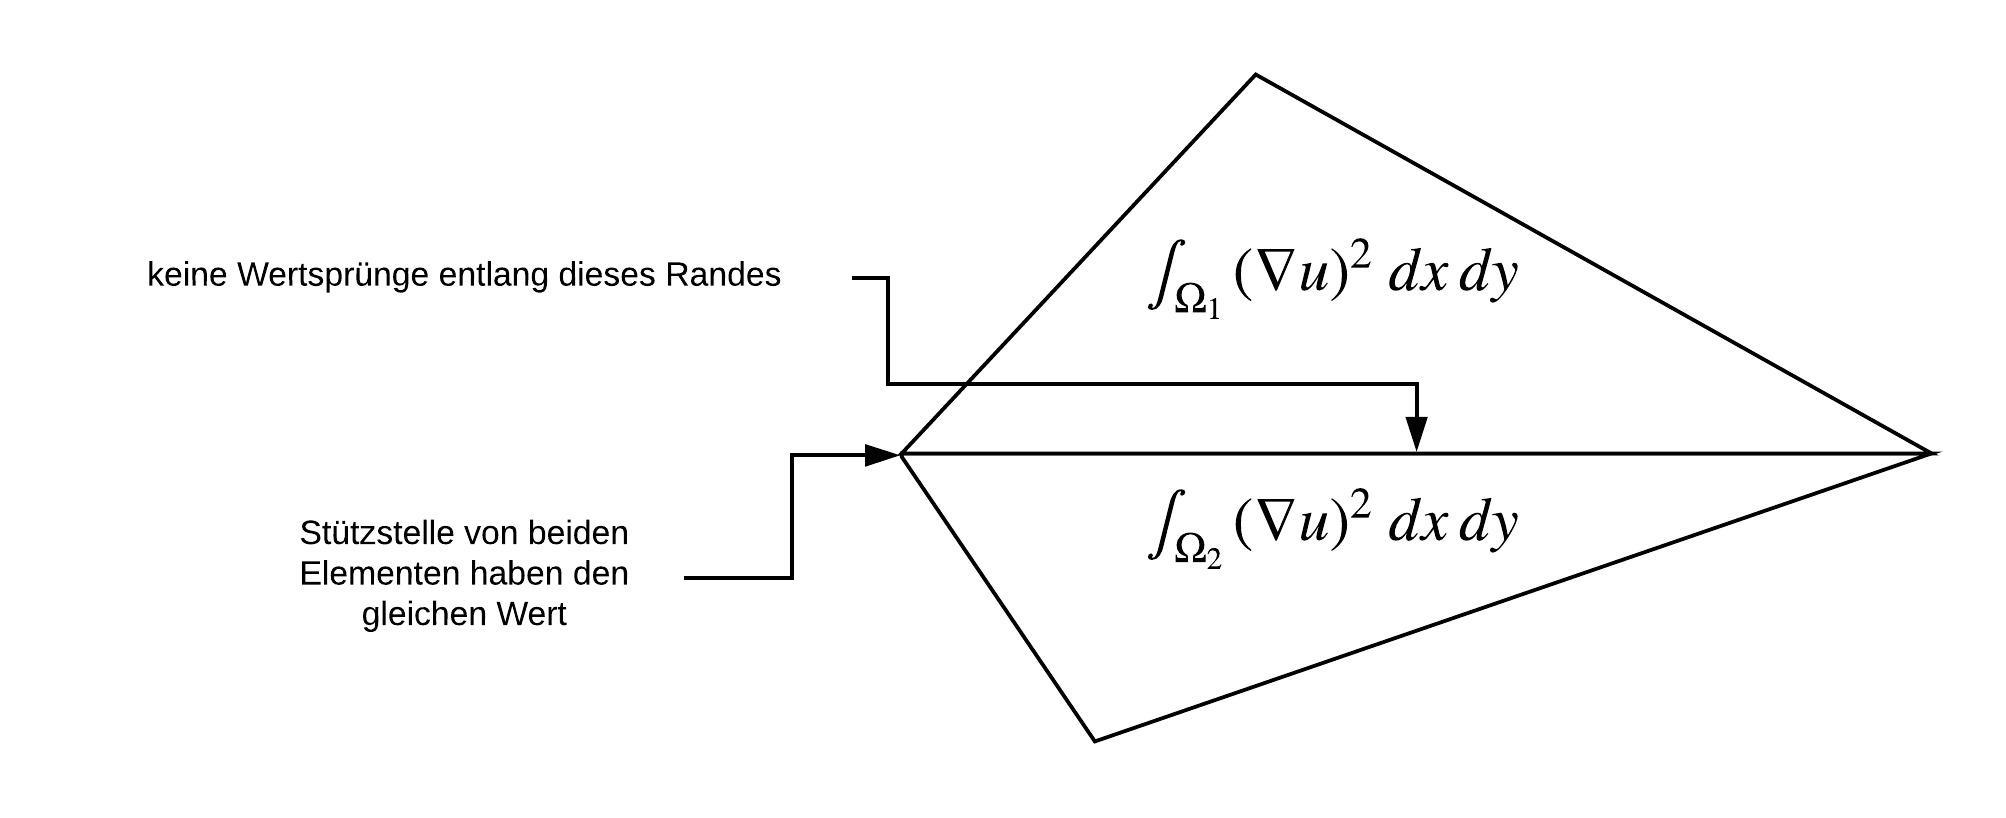
\includegraphics[scale=0.8]{papers/fem/Images/Rand.jpeg}
	\caption{differenzierbar entlang eines Randes}
	\label{fig:Randbedingung}
\end{figure}
Aus der Abbildung \ref{fig:besser Approx} lässt sich erkennen, dass die Ansatzfunktion für jedes Element (Dreieck) unterschiedlich ist. Auch müssen die Ansatzfunktion flexibel auf die grösse des Flächenelements anwendbar sein.
Unteschiedlich zeigt sich im Vergleich der Differential Gleichung mit 1 Dimension und 2 Dimensionen. Die DGL wird folgender massen geändert 
\begin{equation}
	u'' = \lambda u \rightarrow \Delta u = \lambda u 
	\label{fem:DGL2D}
\end{equation} 
während der Laplace Operator die 2. Ableitungen nach den beiden Variablen darstellt.

\begin{equation}
	\Delta = \frac{\partial ^2}{\partial x^2} + \frac{\partial ^2}{\partial y^2}
\end{equation} 
Daraus lässt sich erkennen, dass sich die Vorgehensweise angepasst werden muss, da zweifache Differenzierbarkeit gefordert ist. %Zudem muss die Ansatzfunktion die Approximation genügen genau beschreiben. 
%Poisson-Gleichung:

%\begin{equation}
%\frac{\partial^2 u(x,y)}{\partial x^2} \frac{\partial^2 u(x,y)}{\partial y^2} = - u(x,y)  \in %\Omega
%\label{fem:equation5}
%\end{equation}

%Randbedingungen:
%\begin{equation}
%u = 0, (x,y)\in \Omega
%\label{fem:rand1}
%\end{equation}

%\begin{equation}
%u = U (x,y)\in \Omega
%\label{fem:rand2}
%\end{equation}

%\begin{equation}
%\frac{\partial u}{n} = 0, (x,y)\in \Omega
%\label{fem:rand3}
%\end{equation}
 
%$\Rightarrow$ 4 Parameter $\Rightarrow$ Polynom 3. Grades\\


%\begin{equation}
%\iint_{\!\!\!\!\!\!\!\Omega} \limits (u_2^2 + u_y^2)) \,dx dy
%\label{fem:equation1}
%\end{equation}

%\begin{equation}
%\iint_{\!\!\!\!\!\!\!\Omega} \limits u^2  \,dx dy
%\label{fem:equation2}
%\end{equation}

%\begin{equation}
%\iint_{\!\!\!\!\!\!\!\Omega} \limits u  \,dx dy
%\label{fem:equation3}
%\end{equation}
Aus den Integralen der Teilgebiete muss dann die Lösung gefunden werden, um die Koeffizienten in den Ecken zu bestimmen.
Da es verschiedene Dreieck- Arten gibt sowie auch verschiedene Parallelogramme, wird in Abschnitt \ref{fem:section:loesung} auch eine Lösung aufgezeigt wie mit Hilfe einer Transformation das Dreieck Flächenelements in ein weniger aufwändigere berechenbare Flächenelement überführt werden kann.
Nochmals kurz zusammengefasst was bis hier hin aufgezeigt wurde.
\begin{itemize}
	\item Ebene wird in Teilgebiete unterteilt
	\item Teilgebiete können Dreiecke, Rechtecke oder Parallelogramme sein
	\item Ansatzfunktion soll ein Polynom nierigen Gerades sein
	\item auf jedes Teilgebiet wird eine Ansatzfunktion angewendet
\end{itemize} 
Was bis jetzt noch nicht klar ist, wie die Ansafunktion sich zusammenstellt. Dies wird under anderem im folgenden Kapitel beschrieben.

%\subsection{De finibus bonorum et malorum
%\label{fem:subsection:finibus}}

%\begin{equation}
%\int_a^b x^2\, dx
%=
%\left[ \frac13 x^3 \right]_a^b
%=
%\frac{b^3-a^3}3.
%\label{fem:equation1}
%\end{equation}



